
\chapter{Results}

\section{Objective Result}
\subsection{Without semihard mining}
\begin{itemize}
    \item The distance to the farthest positive stays farther than the one to the closest negative
    \item Possibly due to the outliers in positive instances
\end{itemize}

\begin{figure}[htb]
	\centering
	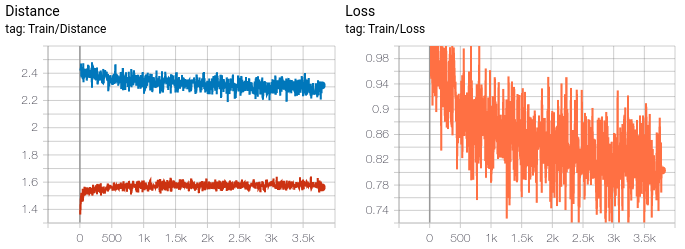
\includegraphics[width=15cm]{Figures/bad_distance.png}
	\caption{The distance to the farthest positive stays farther than the one to the closest negative.}
	\label{bad_distance}
\end{figure}

\subsection{With semihard mining}
\begin{itemize}
    \item Trouble addressed by the use of semi-hard mining. Picking a random positive instead of the farthest while using the closest negative
\end{itemize}

\begin{figure}[htb]
	\centering
	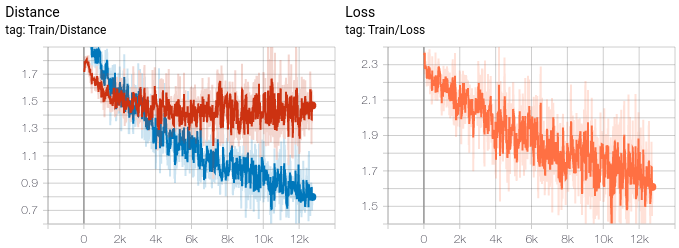
\includegraphics[width=15cm]{Figures/good_distance.png}
	\caption{The distance to the farthest positive becomes closer than the the closest negative on average during the training (with the small dataset)}
	\label{good_distance}
\end{figure}

\begin{figure}[htb]
	\centering
	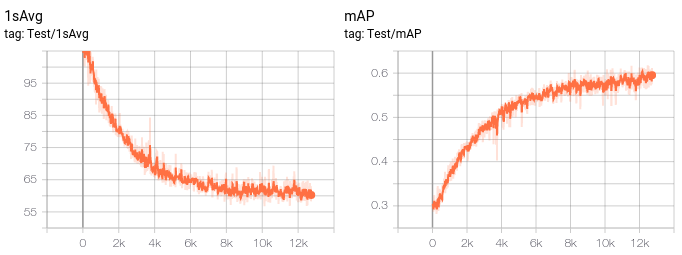
\includegraphics[width=15cm]{Figures/good_semihard_result.png}
	\caption{Left: the rank of positive instances gets lower and lower on average. This means positive instances are projected on closer positions to the anchor instance. Right: mAP (mean average score) increases over the training (with the small dataset)}
	\label{good_distance}
\end{figure}

\section{Subjective Result}

\begin{itemize}
    \item Used the trained model analyzed above to produce audio representations of unseen sounds.
    \item Compared the visualization with OpenL3~\cite{cramer2019} and VGGish model trained with AudioSet ontology~\cite{jort2017}
    \item Applied PCA 2D to the obtained audio representations and visualized them in 2D space
\end{itemize}

\begin{figure}[htb]
	\centering
	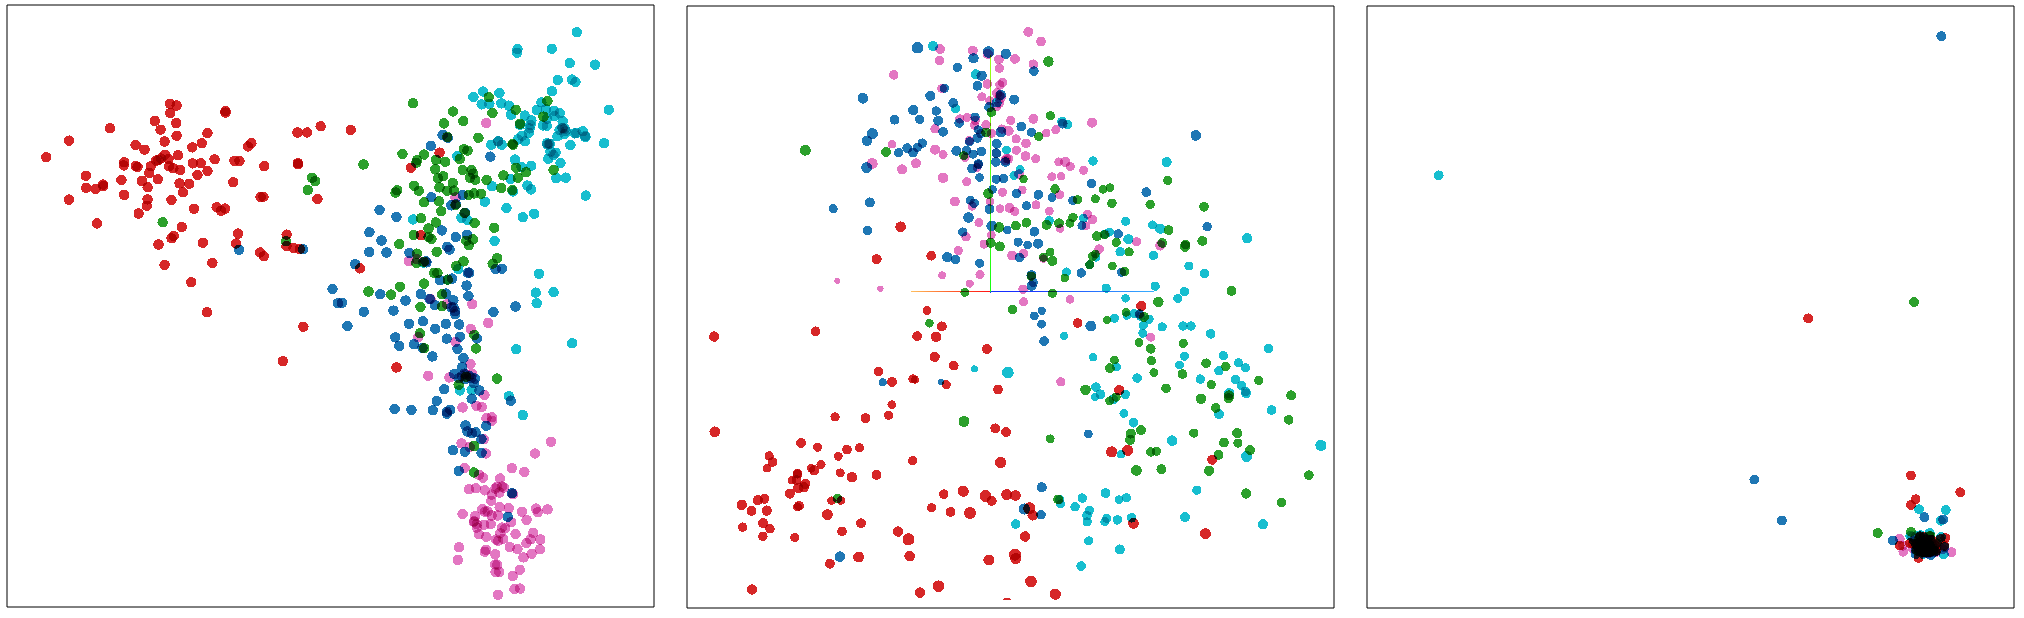
\includegraphics[width=15cm]{Figures/emb_examples.png}
	\caption{Left: Ours (dim 512), Middle: OpenL3 (dim 6114), Right: AudioSet (dim 128) }
	\label{emb_examples}
\end{figure}


\newpage


